\documentclass[11pt]{article}
\usepackage[margin = 1in]{geometry}
\usepackage{amsmath}
\usepackage{amssymb}
\usepackage{amsthm}
\usepackage{graphicx}
\usepackage{enumitem}
\usepackage{url}
\usepackage[parfill]{parskip}
\usepackage{listings}
\usepackage{caption}
\usepackage{subcaption}
\usepackage{mdframed}
\usepackage[utf8]{inputenc}
\usepackage{xcolor}
\definecolor{codegreen}{rgb}{0,0.6,0}
\definecolor{codegray}{rgb}{0.5,0.5,0.5}
\definecolor{codepurple}{rgb}{0.58,0,0.82}
\definecolor{backcolour}{rgb}{0.95,0.95,0.92}
\lstdefinestyle{mystyle}{
	backgroundcolor=\color{backcolour},   
	commentstyle=\color{codegreen},
	keywordstyle=\color{magenta},
	numberstyle=\tiny\color{codegray},
	stringstyle=\color{codepurple},
	basicstyle=\ttfamily\footnotesize,
	breakatwhitespace=false,         
	breaklines=true,                 
	captionpos=b,                    
	keepspaces=true,                 
	numbers=left,                    
	numbersep=5pt,                  
	showspaces=false,                
	showstringspaces=false,
	showtabs=false,                  
	tabsize=2
}
\lstset{style=mystyle}
\newcommand{\skipline}{\vspace{\baselineskip}}
\newcommand{\spacer}{\noalign{\medskip}}
\newcommand{~}{\sim}
\newcommand{\approches}{\rightarrow}
\newcommand{\qarrow}{\quad \rightarrow \quad}
\newcommand{\qqarrow}{\qquad \rightarrow \qquad}
\newcommand{\qtext}[1]{\quad \text{ #1 } \quad}
\newcommand{\qqtext}[1]{\qquad \text{ #1 } \qquad}
\newcommand{\pard}[2]{\frac{\partial #1}{\partial #2}}
\newcommand{\answer}[1]{\textbf{\boldmath #1}}
\newenvironment{problem}[1]{\textbf{Problem: }}{\newpage}

\begin{document}
	
	\begin{center}
		\textbf{Clouds} \\
		\textbf{Stephen Giang} \\
		\skipline \skipline
	\end{center}

	\begin{problem}
		\\
		We need to determine the length, $x$, and amount of overlap, $w$, of $n$ zones, where $n > 0$.  All zones must contain the same length and overlap, and we want the overlap area to not be too large or too small.  From these zones, we will randomly place a cloud in each zone where they will overlap $w$ amount.
		\\ \\
		Notice the following model:
		\begin{figure}[h!]
			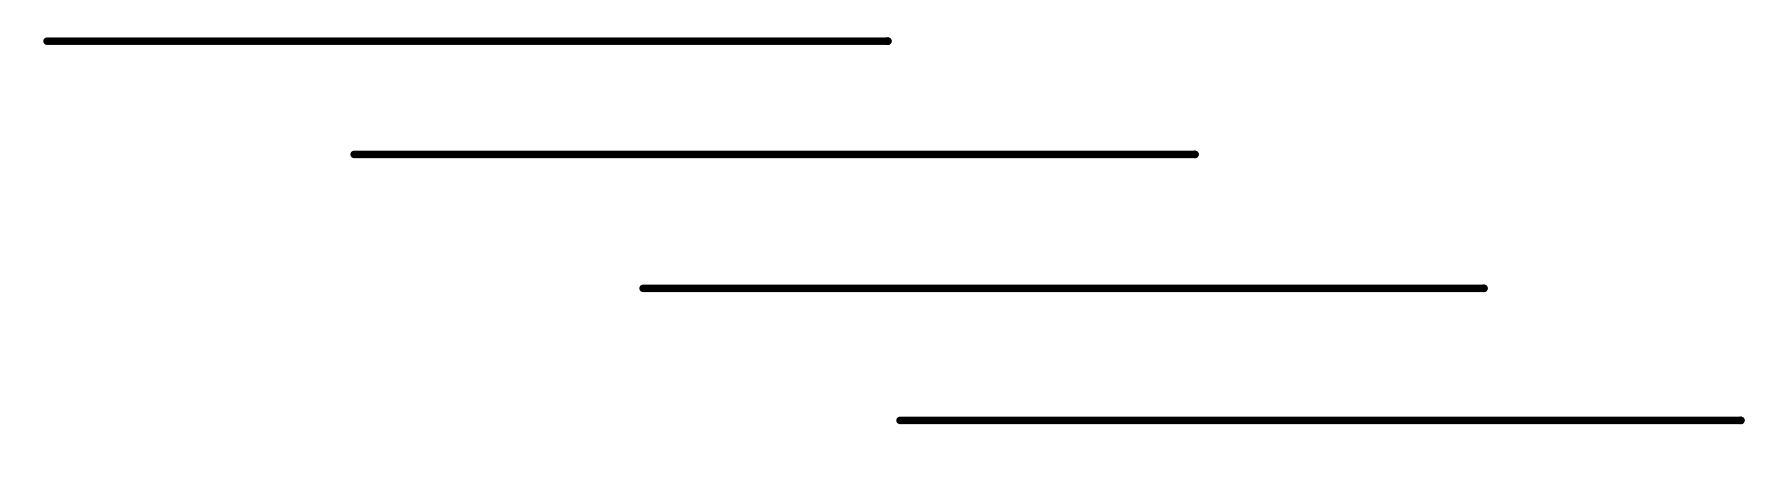
\includegraphics[width=\textwidth]{Model.png}
		\end{figure}
		\\ 
		Each line would represent the area or "zone" that a cloud can be randomly placed.  We can see that they overlap such that the clouds can overlap if placed a particular way.
		\newpage
	\textbf{Solution: }	
		Let $x$ represent the width of each zone, $w$ represent the length of the overlap. We can denote the value of the farthest left point to be 0, and the value of the farthest right point to be 100.
		\\ \\
		We can see that the first line goes from $0$ to $x$.  The second line goes from $x - w$ to $2x - w$.  The third line goes from $2x - 2w$ to $3x - 2w$, and so forth.  This means that for some $n$ amount of zones, we get that that zone goes from $(n - 1)(x - w)$ to $(nx - (n - 1)w)$.
		\\ \\
		Using our given statement that the value of the farthest right point is 100, we see the following:
		\[nx - (n - 1)w = 100\] 
		We can solve for $w$, and get the following:
		\[w = \frac{nx - 100}{n - 1}\]
		We can see that $w$ is a function dependent on $x$.  We now set the range of $w$ to be the following:
		\[\alpha_1x < w < \alpha_2x\]
		where $0 < \alpha_1 < \alpha_2 < 1$.  Using this inequality, we can now find the range of $x$:
		\begin{align*}
			\alpha_1x &< w < \alpha_2x \\
			\alpha_1x &< \frac{nx - 100}{n - 1} < \alpha_2x \\
			\alpha_1(n - 1)x &< nx - 100 < \alpha_2(n - 1)x \\
			\alpha_1nx - \alpha_1x - nx &< -100 < \alpha_2nx - \alpha_2x - nx \\
			(n(\alpha_1 - 1) - \alpha_1)x &< -100 < (n(\alpha_2 - 1) - \alpha_2)x \\
			(n(1 - \alpha_1) + \alpha_1)x &> 100 > (n(1 - \alpha_2) + \alpha_2)x
		\end{align*} 
		From this, we get the following solution:
		\[\frac{100}{n(1 - \alpha_1) + \alpha_1} < x < \frac{100}{n(1 - \alpha_2) + \alpha_2}\]
		\\ \\ \\
	\textbf{Conclusion: } 
		So we have $n$ amount of zones, where each zone is equal in length, $x$, and overlapped the same amount $w$.  We can limit $w$ to only overlap some amount of each zone.  Such that we can range $w$ to be from $\alpha_1 x$ to $\alpha_2 x$.  From this, we can choose $\alpha_1$ and $\alpha_2$ where $0 < \alpha_1 < \alpha_2 < 1$.  Then we can randomly choose some $x$ within the bounds of the above solution, which will allow us to solve for $w$ which will also be within the bounds given above. 
	\end{problem}

\end{document}
